In this section, a novel 3D frame data representation and compression method is described. It was designed to help reduce data size whilst facilitating data processing. This novel representation is named Plane-Tree and is an extension of the basic octree 3D data representation and was inspired by the Shade-Octree (SOT), a data structure developed during in the author's honours thesis \cite{Lincoln13Hons}. More detail about the SOT can be read in \cite{Lincoln13Hons}. \\

The Plane-Tree compresses 3D data and it was also inspired by the Interpolating Leaf Quad-Tree and Shade-Tree representations \cite{Lincoln13Interpolating,Gonzalez07ShadeTree} which are used for image compression. These techniques make use of Quad-Tree decomposition and have been shown to outperform several transform based methods of compression. 

\subsection{Octree Overview}

In this section octree decomposition is explained. This strategy forms a cubic shaped space around some 3D data. In the case of 3D reconstruction, it may be the 3D frame input from an active sensor, stereo method or monocular depth estimation procedure. A geometric representation is then computed for the data contained within the cubic space. This representation may be as simplistic as recording the cube's centre or using the cube to represent the space, or may be complex, employing splines and curvature representation techniques to represent the space. \\

Whatever the representation, a measurement system must be used to decide whether the computed geometric representation adequately fits the data within the space. If the geometric representation is accurate enough for application purposes it may be used in place of the data. This representation is typically designed such that the amount of data required for representation of a space is less than the amount which would be used otherwise. Alternatively, the representation may make use of known correlations which may be more easily compressed than the initial representation. \\


\begin{figure}[!htb]
\centering
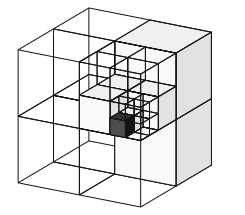
\includegraphics[width=8cm]{images/methodology/pt/octreeVis}
\caption{Visualization of cubic space being split \cite{Hornung13Octomap}.}
\label{fig:SpaceVis}
\end{figure}

If, by the error generated via the measurement system, it is decided the representation is not suitable, the cubic space is broken down into 8 sub-cubes and the process is repeated. For an example of the space broken down into sub-cubes see Figure \ref{fig:SpaceVis}. \\

At each level of decomposition, the data representation achieves finer detail, but more nodes must be stored which means less compression. This is a classic trade-off between compression and accuracy in representing the underlying object. An example of the octree's use in representing an object at differing levels of accuracy is shown in Figure \ref{fig:octreeaccuracy}. In the next section, the decomposition procedure is discussed further. Section \ref{sec:dr:coding} describes the geometric representation employed by the Plane-Tree.


\begin{figure}[!htb]
\centering
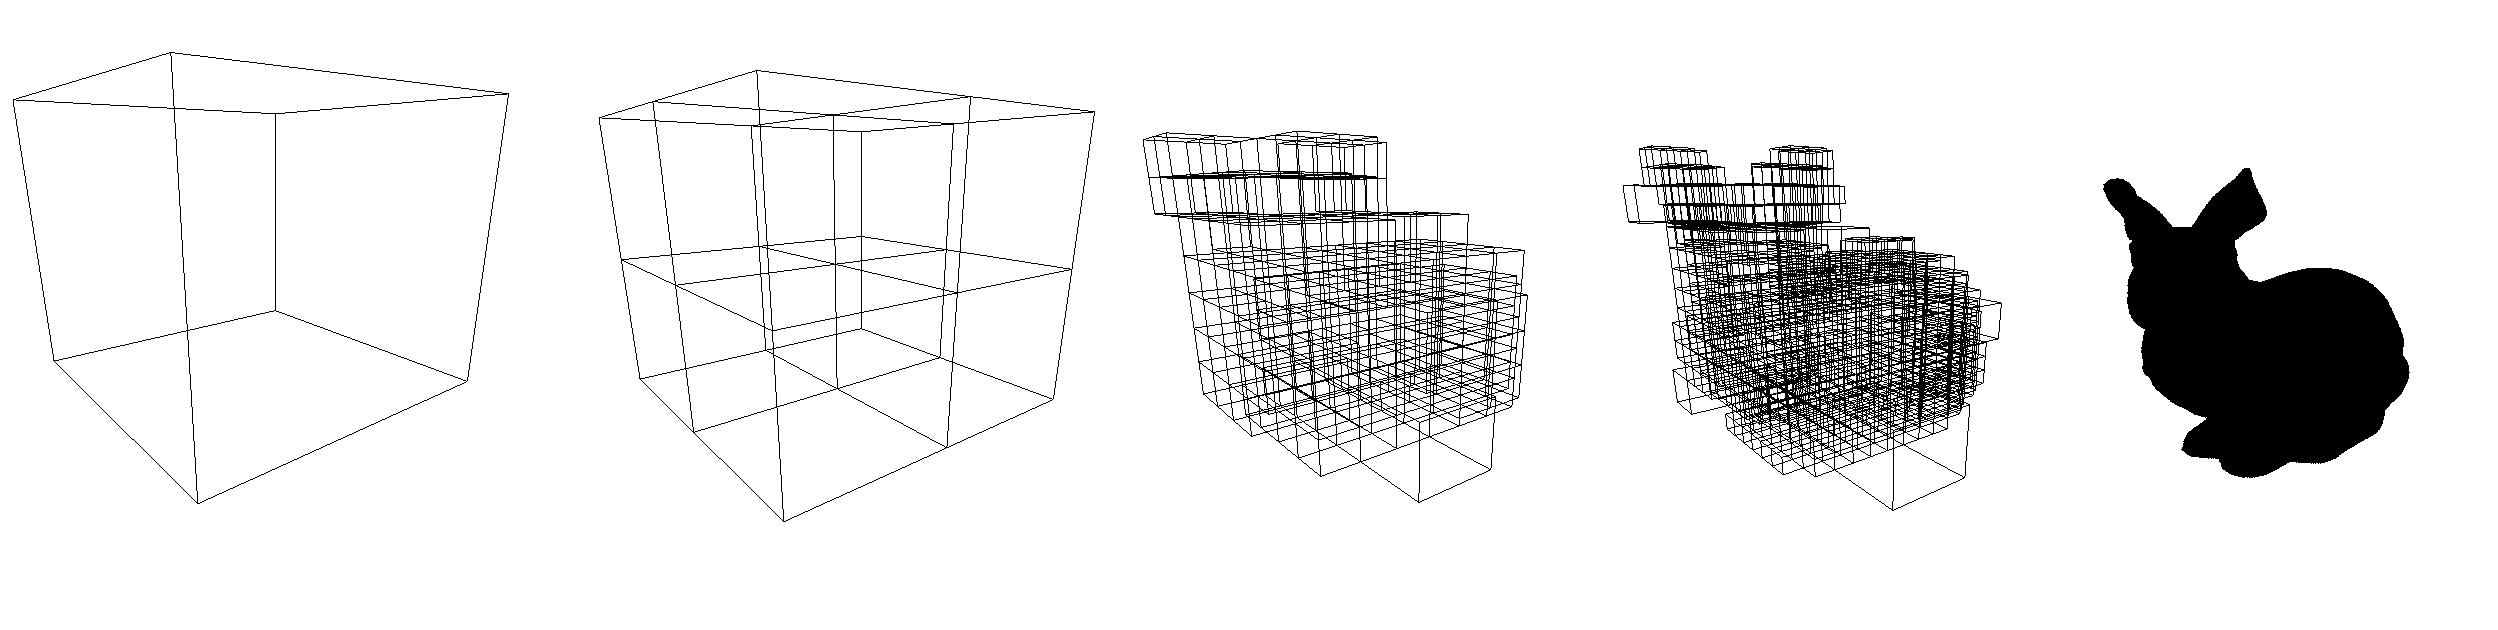
\includegraphics[width=14cm]{images/ch2/OctreeExample}
\caption{An Example of an octree used to represent an object at differing levels of accuracy \cite{Hornung13Octomap}. Left: Original model, Middle: few node splits used to represent the model. Right: many node splits used to more accurately represent the model.}
\label{fig:octreeaccuracy}
\end{figure}


\subsubsection{Octree Description}
\label{OTDesc}

The octree is the three-dimensional extension of the two dimensional Quad-Tree (QT) technique. First we provide some information about the QT and the idea behind using planes or shading the cubic (or square in the case of the QT) nodes to improve compression and efficiency. This was the fundamental idea behind the Shade-Tree and ILQT algorithms \cite{Lincoln13Interpolating,Gonzalez07ShadeTree}. Both these techniques have been shown to improve compression in comparison to state-of-the-art transforms and form the basis of reasoning behind the Plane-Tree. \\

The QT is a hierarchical data structure used for processing and compressing 2D data. Figure \ref{QuadtreeExample} shows an example of a QT used to represent an image. In this figure, the original image is on the left. The QT first uses a single coloured square to represent the entire image, then using some error metric it decides whether to, a) represent the image more accurately using more memory or b) stop decomposition and represent the image with a single colour. If option b) is chosen, the image will look like the second left picture. If option a) is chosen, the image is divided into four sub-images each with its own colour. From here the whole process begins again, with each sub-image given the same options. The final product of the QT is shown on the far right in Figure \ref{QuadtreeExample} and a visualization of a QT hierarchy is shown in Figure \ref{QuadTreeHierarchy}. \\


\begin{figure}[!htb]
\centering
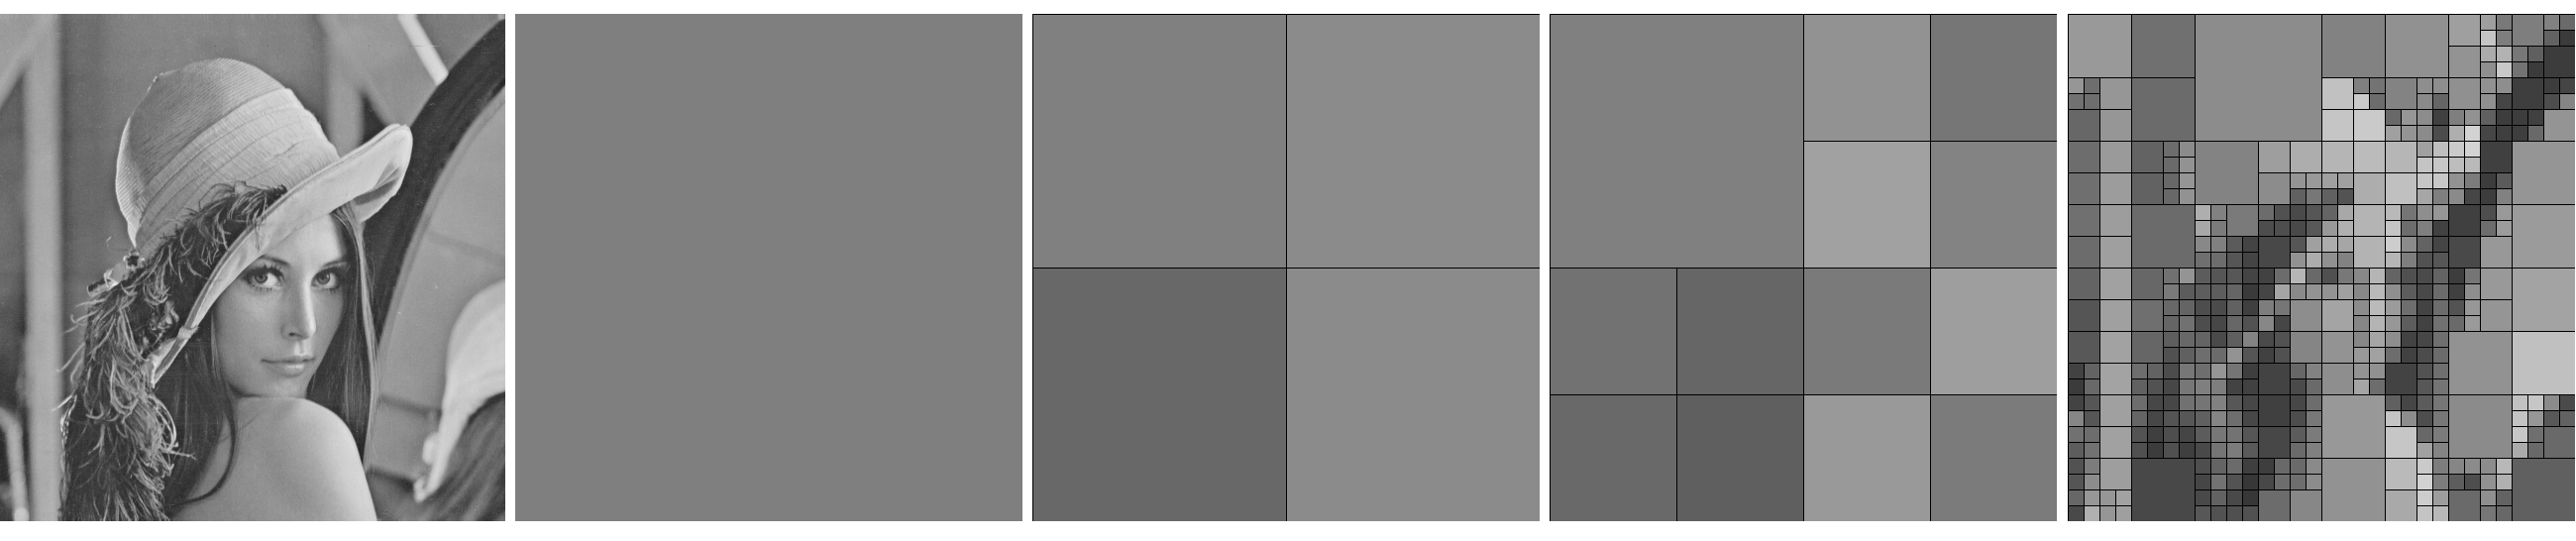
\includegraphics[width=12cm]{images/ch2/quadtreeexample}
\caption{Quadtree Image Representation, left to right: Original Image, 1st Level of Decomposition, 2nd Level of Decomposition, 3rd Level of Decomposition, QT Codec Image.}
\label{QuadtreeExample}
\end{figure}


\begin{figure}[!htb]
\centering
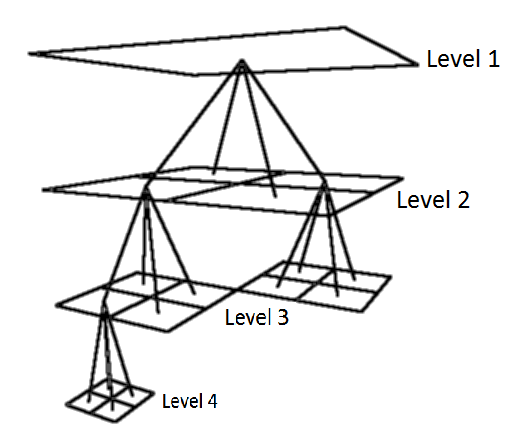
\includegraphics[width=6cm]{images/ch2/QuadTreeHierarchy}
\caption{A visualization of the QT hierarchy}
\label{QuadTreeHierarchy}
\end{figure}

The ILQT and Shade-Tree use small amounts of memory at the corners of the quadrants and interpolate to generate the underlying structure. The small data structures used for representation are much more compressed in their representation than the raw pixel data. For this reason, the ILQT and Shade-Tree do not need to decompose as much as other representations and allow for greater compression as proven by their ability to compete with transform based methods. \\

As mentioned previously, the OT works identically to the QT but in 3D. Instead of surrounding the 2D image with a square encompassing the entire frame, a cube is used to enclose the 3D space. Similar to the QT method, an error metric is used to decide whether the current representation is adequate. If the octant must be split, it is divided into eight sub-octants. Each split operation divides each coordinate ($x,y,z$) by two, giving the 8 sub-octant spaces. Figure \ref{OctreeExample} shows an example of this decomposition process. The further each cube is split, the more the OT resembles the model being compressed. In the QT and OT, nodes which have not been split are called leaf nodes and the function which decides whether a node should be split is called a leaf criterion function. \\ 

\begin{figure}[!htb]
\centering
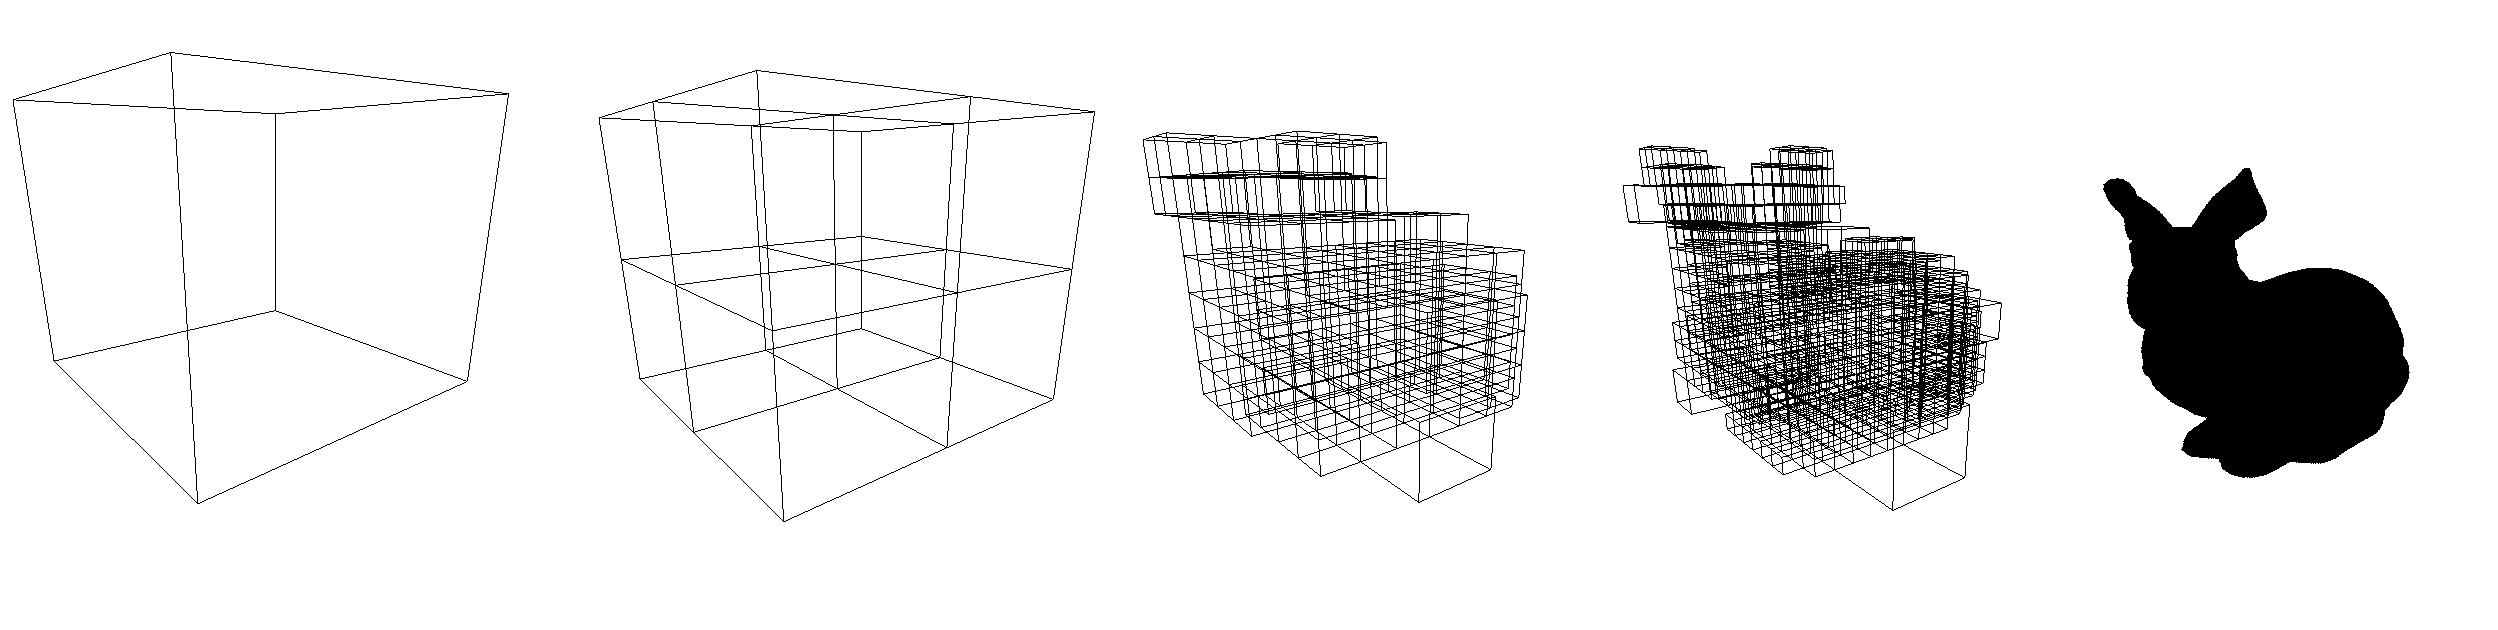
\includegraphics[width=16cm]{images/ch2/OctreeExample}
\caption{Visualization of OT Decomposition}
\label{OctreeExample}
\end{figure}

The goal of the OT and the QT is to implicitly store the size and attributes of each node. There are two main methods of representation, a packed traversal of the tree and a linear tree. The packed traversal method stores the hierarchy using a pre-defined traversal of the tree, and typically follows one of two orderings. These are, breadth-first traversal and depth-first traversal, as seen in Figure \ref{TreeTraversalExample}. The depth-first traversal starts at the root, then works it's way down, top to bottom, then left to right of the tree. In essence, it travels to a node's children before considering its neighbours. In contrast, the breadth-first traversal goes to all nodes which are at the same depth before continuing to lower levels. \\


\begin{figure}[t]
\centering
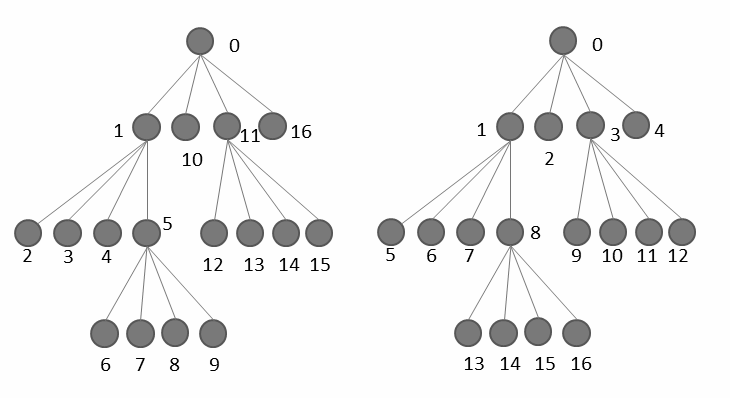
\includegraphics[width=12cm]{images/ch2/TreeTraversalExample}
\caption{Tree Traversals, Left: Depth-First Traversal, Right Breadth-First Traversal}
\label{TreeTraversalExample}
\end{figure}

Encoding the two packed tree traversal methods requires one nibble (4 bits) for a QT node, and one byte (8 bits) for an OT node. Here, the bits represent the structure of the sub-node. For example, the QT node bit sequence, $1001_2$ means that the node has two children (corresponding to the ones), the sequence $0000_2$ means the node is a leaf node. Each bit position indexes a child node using a pre-determined ordering. An example of a possible ordering for a quadrant and an octant is shown in Figure \ref{ChildOrderExample}, both breadth-first and depth-first traversals use the same index method, the difference lies only in the order in which nodes are visited. 

\begin{figure}[!htb]
\centering
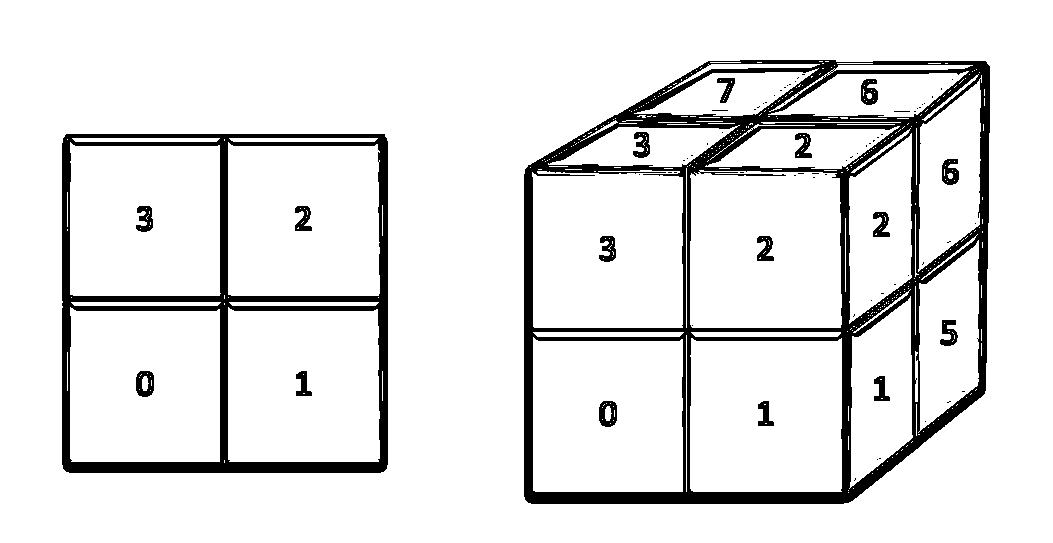
\includegraphics[width=12cm]{images/ch2/ChildOrderExample}
\caption{A possible child ordering for the QT (left), and the OT (right).}
\label{ChildOrderExample}
\end{figure}

The linear tree representation stores each leaf node individually. Each leaf is encoded as the pathway from the root to the leaf itself. This method was investigated in the 1980s \cite{Gargantini82Effective,Yufei88Octcodes}, but has not been used much in modern compression algorithms due to its inefficiency compared with the packed traversal method. An example of this structure is shown in figure \ref{LinearCellCodeRepresentation}, where each node: $a$, $b$, $c$, $\dots$ , $m$  is encoded as a variable length traversal path. The QT and OT are widely used in image \cite{Varma12Application} and 3D compression \cite{Schnabel06Octree}. Hanan Samet \cite{Samet88Fund1} presents an introduction to both structures, he also describes both tree storage methods in depth. 

\begin{figure}[!htb]
\centering
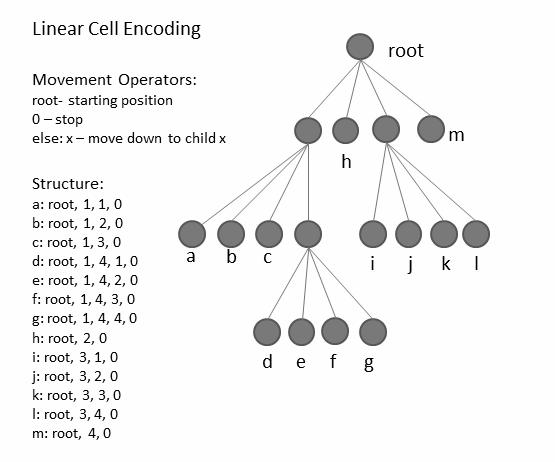
\includegraphics[width=12cm]{images/ch2/LinearCellCodeRepresentation}
\caption{A Linear Tree Code Representation Example}
\label{LinearCellCodeRepresentation}
\end{figure}



\subsection{3D ShadeTree Coding}

\label{sec:dr:coding}

The Shade-Tree compression system \cite{Gonzalez07ShadeTree} was designed for the compression of 2D image data. However, this method is easily extended to 3D Volumetric data. In this system, octants are decomposed in the same manner as with a regular octree but the leaf node representation is different. In the Shade-Tree system, the corner values in the volume are sampled for each node.  \\


To model the geometric information within each node using the corner values, interpolation is used. By interpolating between the 4 corner values, a model of the data within the geometric subspace within the node may be generated. This representation saves space by storing only 4 corner values rather than explicitly storing the dense volumetric data. As in the 2D Shade-Tree, this method allows nodes to share data and further compress the structure. For example, if two leaf nodes happen to share a corner, then the corner only needs to be encoded at the node which is visited first according to the ordering of the tree (breadth-first or depth-first). This constitutes no additional coding for the representation. \\

The Shade-Tree coding method can quantize the corner values and map them into values within the range $[0,255]$. This way the Shade-Tree requires four or fewer bytes per leaf node. The Shade-Tree is ideal for 2D images or volumetric 3D data. In this research I aim to target sparse 3D volumetric and sparse 3D mesh data. Therefore, another data structure based on the octree, the Plane-Tree is proposed. This data representation is similar in idea to the Shade-Tree but was designed for low bit-rate compression of sparse 3D data as well as occupancy grids which are commonly generated by 3D reconstruction algorithms. \\

%This data representation may also be used to represent Signed Distance Functions, which are now commonly used in 3d reconstruction as a means of representation. In fact, such a scheme would greatly benefit the compression method of the Shade-Tree since its data is typically represented as smooth changes along a given path. \\

\subsection{Plane-Tree Coding}

The proposed Plane-Tree method is also based on octree subdivision. The technique places the input 3D frame/mesh or volume into a cubic space. It checks whether the representation corresponding to this single cube is at a desired level of quality. If it is not, the cube is decomposed into 8 sub-cubes. For each sub-cube associated with the 3D data, the process repeats. This process is further controlled using an error threshold and a maximum depth value. At each level of subdivision, the error between the sub-cube (or node) representation of the space is compared to the original geometric information within the sub-space of the cube. If the error is below the error threshold, decomposition stops. This way, the desired level of accuracy can be more easily controlled rather than manually inspecting the quality prior to subdivision. Likewise, the level of subdivision may freely continue until the maximum tree depth is reached, this also assists in controlling the quality vs. compression ratio. To this end, the depth of each node is compared to the maximum depth. If the maximum depth is reached, decomposition stops and other nodes are visited until the procedure ends. \\

In the typical octree node representation, the raw cube is used to represent the space. Unless this cube is small (deep within the tree) the error is typically high. Trees which are very deep require more storage space. Our method stores arbitrary first order planes within nodes at 20 bits per leaf. This small bit cost per leaf node greatly improves compression performance compared to the octree and makes it competitive with state-of-the-art methods. \\

 
In the following sections, we present the details of the Plane-Tree in terms of subdivision, leaf node plane computation and representation as well as compression and decompression. \\


\subsection{Octree Subdivision}

Prior to compression, the input 3D model is normalized into a $512^3$ space. Starting with the cube which represents the entire space, a 3D Plane representation is computed based on the data within the cube. The mean squared error metric is computed between the sampled points of the plane and the sampled points of the 3D object (which lie within the cube). If this value is below a given threshold, or the maximum level of subdivision is reached, decomposition stops. Alternatively if both predicates (maximum depth and error threshold) are not met, the cube is divided into 8 sub-cubes. Each sub-cube is then tested to see whether part of the mesh lies within it. If so, the process it repeated for that cube, otherwise no further action is taken. \\

Each cube/sub-cube is referred to as a node. Each node which has no children is referred to as a leaf node. During compression/decompression, the plane based representation is only stored at leaf nodes, with non-leaf nodes serving only as paths giving the location of leaf nodes. Below, the computation and representation of our novel leaf node data model is discussed. \\

\subsection{Leaf Node Computation and Representation}
\label{NRep}

Our novel leaf node representation better represents the mesh which intersects it than the octree, it does so by using a first order plane. This representation requires only 20 bits, allowing it to encode higher quality models whilst saving on bits which would otherwise be used to form a deeper, and thus more costly, octree representation. This also gives the Plane-Tree an advantage at low bitrates. \\

To generate a plane for a given leaf node, we first sample the mesh within the node space. Using these points, the x, y and z axis variances are measured. These indicate how much variation lies across each axis within the node. We then find the plane using least squares, solving for the axis with the lowest variance. Once we have coefficients describing the plane, we use a single point on the plane, and the plane normal to describe it. \\

Using a point on the plane and a plane normal, we can find a set of triangles which represent the plane within the node. We first find all points in which the cube's edges intersect with the computed plane. Using the average point as the origin, and the plane's normal as the y-axis, we order the points based on their x/z angle. This gives us an ordered set of points which corresponds to a polygon defining the plane within the node. This polygon is then triangulated forming the final representation. This process is used at both the compression and decompression stages. \\

The triangles representing the plane within the node are then sampled along with the parts of the mesh lying within the node. The mean squared error (mse) is then taken between these samples for comparison with the error threshold value. Within the summation for the mse we use the closest point within the second point set, this is shown in equation \ref{eqn:MSE_1}.

\begin{equation}
 \label{eqn:MSE_1}
MSE(pts_1, pts_2) = \frac{1}{N}\sum_{i=0}^{N} (pts_{1_i} - closest(pts_{1_i}, pts_2))^2
\end{equation}

Using this equation, the sampled points from the plane triangles $p$, and the sampled points from the mesh $m$ (which lie within the cube), we take the average of both mean squared errors as a measurement of total error, $error = \frac{1}{2}MSE(p,m) + \frac{1}{2}MSE(m,p)$. This is the value which is compared with the error threshold to decide whether decomposition should stop. \\

To compress the data for our leaf node representation, we store the plane using its normal vector and a single point lying on the plane. We store the normal vector using 12 bits (4 bits per coordinate). The point which lies on the plane is represented using two pieces of information, an edge number and a distance variable. It must be mentioned that for a given plane which intersects a cube, a minimum of 3 of the cube's edges pass through the plane. We therefore record one of these edges (the edge number) and the distance from on of its end points (the distance variable). Each edge has a predefined number which identifies it, all edges also have a predefined start and end point. \\

Each cube has 12 edges in total, so 4 bits are used for the edge number, another 4 are used for the distance variable. Adding these to the normal vector results in 20 bits per leaf node representation.  \\


\subsection{Compression and Decompression}

To compress our data structure we iterate through the tree in depth-first order. If we encounter a non-leaf node, we first store a single bit of $1_2$. Then the configuration of the sub-nodes (since not every sub-node intersects the object) is stored as a single byte. Each bit is labelled $1_2$ if a particular sub-node exists and $0_2$ if it does not. This is possible since we order our sub-nodes in a predefined order. If a leaf node is encountered, we store a $0_2$, then record our 20 bit leaf node representation in three other files: the normal data, the distance variables and edge numbers, totalling 4 files (tree, normals, distances and edge numbers). After the entire structure is stored we employ entropy encoding on each of these files. \\

To decompress our structure, we read the first bit of the output file. This step checks if the current node is a leaf or not. If it is, we read out a 20 bit plane representation (from the three separate files) and generate a list of triangles representing where the plane intersects the node (explained in section \ref{NRep}). These triangles are then added to a final database which represents the decoded model. If we reach a non-leaf node, we read out the 8 bit sub-node configuration and repeat the process for each existing sub-node in the predefined order. \\  
